\chapter{Kadio Company Ltd}
\section{KD-350MS}\index{KADIO!KD-350MS}
Calcolatrice prodotta in Cina dalla Kadio Company Ltd~\cite{wiki2021} , clone Casio FX-350MS\index{Casio!FX350MS}
\subsection{Test interno}
Il test\[\arcsin(\arccos(\arctan(\tan(\cos(\sin(9))))))=9\] ha come risulta dalla tabella~\vref{tab:KADIOKD350MS}. 
\subsection{PCB}
Sigla PCB:KD82MS-4 2015.06.10
\subsection{Modi funzionamento}
La calcolatrice ha tre modi di funzionamento, calcoli aritmetici di base, deviazione standard, calcoli di regressione
\subsection{Formati visualizzazione}
Premere tasto \tastomode finché si ottiene la schermata
\begin{center}
	\CASIOmodediplayexp
	
\end{center}
\begin{description}
	\item[\tasto{1} FIX]Numero cifre decimali
	\item[\tasto{2} SCI]Numero cifre significative
	\item[\tasto{1} NORM]Formato di visualizzazione decimale
\end{description}
\subsection{Angoli}
Premere tasto \tastomode finché si ottiene la schermata
\begin{center}
	\CASIOmodediplayang
	
\end{center}
\begin{description}
	\item[\tasto{1} Deg]Gradi
	\item[\tasto{2} Rad]Radianti
	\item[\tasto{1} Gra]Gradi Centesimali
\end{description}
\begin{table}
	\centering
	\begin{tabular}{lll}
		\toprule
		\multicolumn{1}{c}{Modello}&\multicolumn{1}{c}{Risultato}&\multicolumn{1}{c}{Errore}\\
		\midrule
		KADIO KD-350MS&\num{8.9999999998}&\num{1.921103e-9}\\
		\bottomrule
	\end{tabular} 
	\caption{KADIO KD-350MS}
	\label{tab:KADIOKD350MS}
\end{table}
\begin{table}\centering
	\begin{tabular}{ccc}
		\toprule
		MODO	&TASTI  &  DISPLAY\\ 
		\midrule 
		Calcoli aritmetici di base	& \tastomode\tasto{1} & COMP \\ 
		\midrule 
		Deviazione standard	&\tastomode\tasto{2}  & SD \\ 
		\midrule 
		Calcoli di regressione	&\tastomode\tasto{3}  & REG  \\ 
		\bottomrule
	\end{tabular} 
	\caption{Modi:KADIO KD-350MS}
	\label{tab:KADIOKD350MSModi}
\end{table}
% TODO: \usepackage{graphicx} required
\begin{figure}
	\centering
	\includegraphics[width=0.5\linewidth]{"kadio/kadio kd-350ms"}
	\caption[KD-350ms front]{}
	\label{fig:kadio-kd-350ms2}
\end{figure}

%\begin{figure}
%	\begin{subfigure}[b]{.5\linewidth}
%		\centering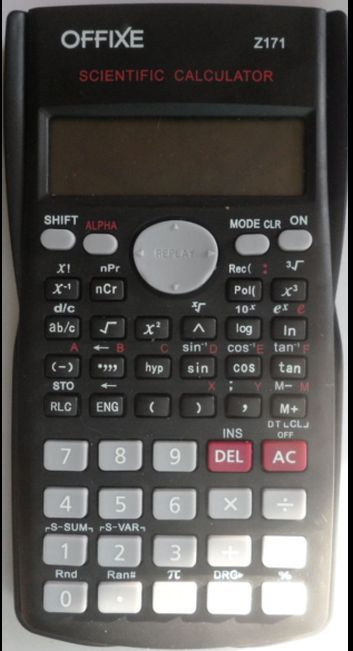
\includegraphics{offixe/SAM_3719}%
%		\caption{Fronte}\label{fig:OFFIXEfront}
%	\end{subfigure}%
%	\begin{subfigure}[b]{.5\linewidth}
%		\centering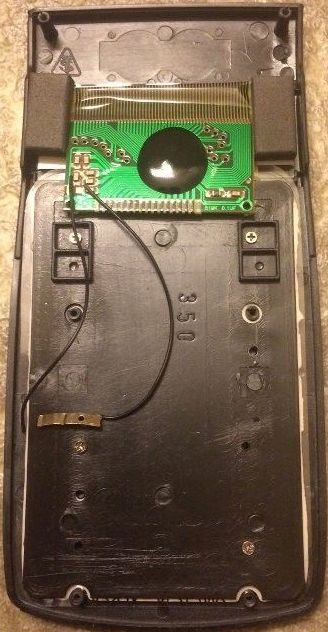
\includegraphics{offixe/7019561509344433257}%
%		\caption{PCB}\label{fig:OFFIXEPCB}
%	\end{subfigure}
%	\caption{OFFIXE KD-82MS (Z171)}\label{fig:OFFIXEKD82MS}
%\end{figure}
